\documentclass[a4paper,12pt]{article}
\usepackage[]{amsmath}
\usepackage[UTF8]{ctex}
\usepackage{geometry}
\usepackage{tikz}

\newcommand\tikzmark[1]{%
\tikz[overlay,remember picture] \node[coordinate] (#1) {};%
}

\begin{document}
    \title{狄拉克旋量}
    \author{李成蹊\\中国科学院物理研究所}
    \maketitle
    \section{旋量简介}
    旋转轴是类似于张量的数学实体,可以对旋转和洛仑兹Boost下的不变性的概念进行更一般的处理。对于每一个$k$阶张量都对应于一个$2k$阶旋量,并且一些张量可以与相同阶旋量联系起来。例如一个广义上的四维矢量可以对应于2阶厄米旋量,可以用$2\times 2$的厄米矩阵来表示。一个零四维矢量也可以与一个一阶旋量联系起来,也能表示成两分量复向量。我们将会在下文看到。

    旋量也能在非相对论情形下应用,但是它在洛伦兹变换下自然的出现。可以说旋量是洛伦兹变换的最基本的数学对象。

    1897年,克莱恩(Klein)最初设计旋量是为了简化经典陀螺的处理。人们认为1913年的艾利·卡丹(Elie Cartan)更透彻地将旋量作为数学对象进行了研究。它们与哈密尔顿四元数密切相关。

    当人们发现电子和其他粒子有一种叫做“自旋”的角动量的固有形式时,自旋子开始在物理学中扮演更广泛的角色,而这种角动量的行为被Cartan发现的数学方法正确地捕捉到了。泡利在一个非相对论性(即低速)的环境中形式化了这种联系,用一个双组分复矢量对电子自旋进行了建模,并引入了泡利自旋矩阵。然后,在寻求与洛伦兹协变性要求一致的描述电子的量子力学描述时,保罗·狄拉克(Paul Dirac)有一个精辟的见解,即如果将数学里的旋量与现有的量子力学波函数相结合来描述电子,则可以找到正确形式的方程。他引入了现在被称为狄拉克旋量的四分量复向量,并且物理上解释了这样获得波函数,他预言了反物质的存在。

    这里我们更一般的讨论旋量,关注于最简单的情况,也就是2分量旋量。这些足以描述三维的旋转,和三维+一维的洛伦兹变换。我们将会简短的介绍高阶旋量,它们的变换类似于一阶旋量。然后我们将会介绍狄拉克的理论,它可以被看成一对一阶旋量的耦合方程。

    在非相对论量子力学和自旋角动量的处理中,本科生经常首先遇到旋量。这可以给人的印象是,旋量本质上是关于自旋的,这是一个强化的名字“旋量”的印象。然而,你应该在一开始就尽量避免这种假设。把“旋量”这个词看作是“矢量”或“张量”的概括。我们将会遇到一个描述电的4-电流的旋量,例如,和一个法拉第张量的旋量版本,从而用旋量符号写出麦克斯韦方程组。

    就像我们可以把矢量想象成空间中的箭头,把四矢量想象成时空中的箭头一样,画出一个1阶旋量的几何图形也是很有用的(或者简称为“旋量”):参见图1。它可以被描绘成一个有两个特征的向量:一个在空间中选择包含这个向量的平面的“旗子”和一个整体的符号。关键的特性是,在旋转的作用下,旋量的方向会像矢量一样发生变化,而旗子的移动方式与它被刚性地固定在旗杆上是一样的。绕着旗杆轴旋转对向量在空间的指向没有影响,但是对旋量却有影响,因为它转动了旗帜的方向。
\begin{center}
    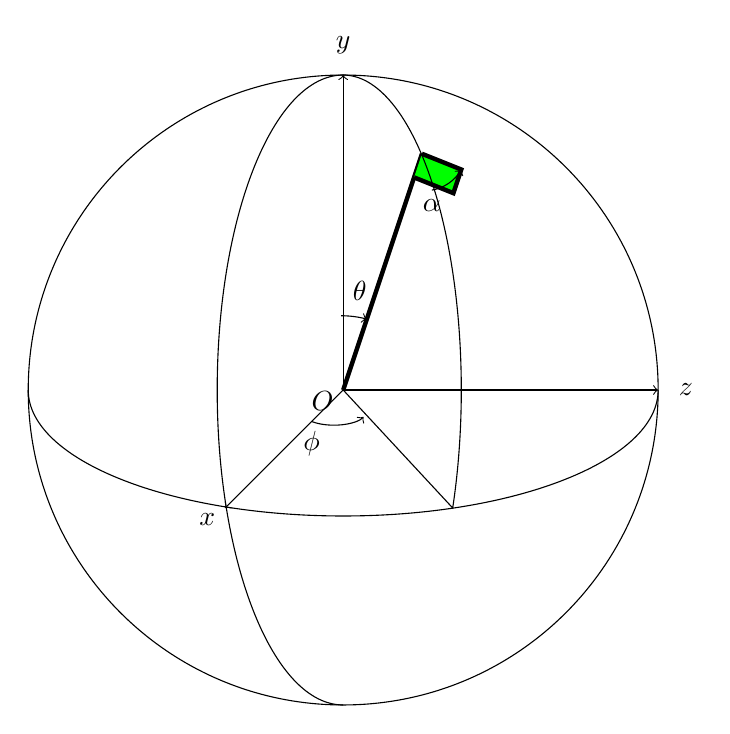
\begin{tikzpicture}
        \draw[->] (0,0) -- (4,0) node[right=4pt]{$z$};
        \draw[->] (0,0) -- (0,4) node[above=4pt]{$y$};
        \draw[->] (0,0) -- (-1.5,-1.5) node[below=4pt,left]{$x$};
        \node[below=4pt,left] at (0,0) {$O$};
        \draw (0,0) circle (4);
        \draw (0,4) arc (90:270:1.6 and 4);
        \draw (4,0) arc (0:-180:4 and 1.6);
        \draw[ultra thick] (0,0) -- (1,3);
        \filldraw[fill=green,ultra thick] (1,3) -- ++(0.5,-0.2) -- ++(-0.1,-0.3) -- +(-0.5,0.2);
        \draw[<-] (0.3,0.9) arc (75:90:1.264);
        \node[right] at (0,1.264) {$\theta$};
        \draw (0,4) arc (90:-22:1.5 and 4) -- (0,0);
        \draw[->] (-0.4,-0.4) node[below]{$\phi$} arc (-135:-20:0.4 and 0.16);
        \draw[<-] (1.5,2.8) arc (-30:-80:0.54) node[below]{$\alpha$};
    \end{tikzpicture}\\
    图1
\end{center}

    旋量的整体特征更加微妙。我们将会发现,当旋量转动$2\pi$,如我们所预料一般,回到了原来位置。但它也有一个整体的符号变化。你可以认为这类似于相因子($e^{i\pi}=1$)。当一次考察一个旋量时,这个符号没有任何后果,但当一个旋量与另一个比较时,它可能是有关的。当我们使用一对复数(一个2分量的复数向量)来引入数学描述时,这个特性和所有其他特性都会自动被考虑进去。

    确定一个旋量必须提供四个实参数和一个符号:在图1里给定了一个合理的参数集$r,\theta,\phi,\alpha$。人们可以看到,如果想要分析旋量的运动,就会很自然地提出这样一个集合。除非另有明确说明,否则我们将假定整体符号为正。在经典陀螺上的应用是这样的:旋量可以表示陀螺的瞬时位置状态。然而我们对这种应用没有兴趣。在这篇文章里我们将会看到旋量可以用来表示无质量粒子的能量动量和自旋,并且一对旋量可以用来表示有质量粒子的能量动量和泡里-罗巴斯基自旋。自旋角动量的一些非常有趣的性质,在其他情况下可能看起来很神秘,但当我们使用旋量时,它们会自然地出现。

    旋量类似于矢量可以被旋转。在旋转操作下,旋量大小固定,但角度$\theta,\phi,\alpha$却改变了。在图里,旗杆和旗帜一起组成一个刚体;这就可以确定$\alpha$如何随着$\theta$和$\phi$改变。为了写出确定的旋转方程,很方便的做法是把四个参数写到两个复数里。
    \begin{equation}
        \begin{aligned}
            a & \equiv \sqrt{r} \cos (\theta / 2) e^{i(-\alpha-\phi) / 2} \\
            b & \equiv \sqrt{r} \sin (\theta / 2) e^{i(-\alpha+\phi) / 2}
        \end{aligned}
    \end{equation}\label{spin1}
    之所以用根号和因数$1/2$的原因在后面讨论中会显而易见。旋量绕着$y$轴旋转$\theta_r$角表示为
    \begin{equation}
        \left(\begin{array}{l}
            a^{\prime} \\
            b^{\prime}
            \end{array}\right)=\left(\begin{array}{cc}
            \cos \left(\theta_{r} / 2\right) & -\sin \left(\theta_{r} / 2\right) \\
            \sin \left(\theta_{r} / 2\right) & \cos \left(\theta_{r} / 2\right)
            \end{array}\right)\left(\begin{array}{l}
            a \\
            b
        \end{array}\right)
    \end{equation}\label{spin2}
    当我们研究下面更一般的转动时,我们将证明这个表达式。

    从现在起,我们将提到双分量复向量
    \begin{equation}
        s=s e^{-i \alpha / 2}\left(\begin{array}{c}
            \cos (\theta / 2) e^{-i \phi / 2} \\
            \sin (\theta / 2) e^{i \phi / 2}
            \end{array}\right)
    \end{equation}\label{spin3}
    作为一个旋量。旋量的尺度$s$表示旗杆的长度。
    \begin{equation}
        r=|a|^{2}+|b|^{2}=s^{2}
    \end{equation}\label{spin4}
    旗杆矢量的空间分量$(r_x,r_y,r_z)$分别表示为
    \begin{equation}
        r_{x}=a b^{*}+b a^{*}, r_{y}=i\left(a b^{*}-b a^{*}\right), r_{z}=|a|^{2}-|b|^{2}
    \end{equation}\label{spin5}
    可以通过带入\eqref{spin1}来证明上式。现在你可以看到为什么\eqref{spin1}里需要用根号表示。

    复数表示将被证明是理解旋量的核心。它给出了一个旋量的第二个图像,一个二维复向量空间中的向量。应该学会把这两种图像放在一起学习。大多数人发现他们自己在三维真实空间中形象地思考国旗,如图1所示。但时不时地提醒自己,在复向量空间中,一对相反的旗杆状态,如“沿z向上”和“沿z向下”是互相正交的。(你可以从\eqref{spin3}里看到,当z方向向上或向下时,复向量分别为$(s,0)$和$(0,s)$).

    图二给了一些旋量复数表示的例子。值得注意,两个基本矢量$(1,0)$和$(0,1)$分别与旗杆$z$方向向上和$z$方向向下分别对应。作为复向量来考虑,它们相互正交,但是它们在三维空间中的方向则是互相反向。换句话说,复自旋空间里转动$\theta_r$对应于三维实空间的$2\theta_r$的转动。这被称之为二倍角度关系,也可以从\eqref{spin3}里看到。

    绕$y$轴转动矩阵\eqref{spin2}是实的,所以由$(1,0)$绕$y$轴转动获得的所有旋量态都是实的。这些所有与$y$轴满足右手关系的旗帜和旗杆都在$xz$平面。绕$z$轴转动矩阵可以表示为对角矩阵。为了寻找这个对角矩阵,我们考虑沿着$x$轴正方向的旋量$(1,1)$。绕$z$轴旋转应该使得$\phi$增加$\theta_r$. 这意味着旋量绕$z$轴旋转$\theta_r$的矩阵为
    \begin{equation}
        \left(\begin{array}{cc}
            \exp \left(-i \theta_{r} / 2\right) & 0 \\
            0 & \exp \left(i \theta_{r} / 2\right)
            \end{array}\right)
    \end{equation}
    当我们把它作用在$(1,0)$上式,结果为$(e^{-i\theta_r/2},0)$。这表示这个结果是把$\alpha+\phi$增加了$\theta_r$. 因此,旗帜转动了。为了与旋量方向绕$z$轴转动保持一致,把它解释成$\phi$的改变而$\alpha$的不变是有道理的。

    迄今为止,我们旋量的图像纯粹是一个空间性的。我们习惯于通过找到第四个量并形成一个四向量来将三向量放入时空。然而,对于旋量,则使用另一种不同的方法,因为它将证明旋量已经是一个时空对象,可以被洛伦兹变换。要将旋量“放置”在时空中,我们只需要找出它所在的三维区域或“超曲面”。我们将会在后面看到,与旗杆联系的四矢量是零矢量。因此,旋量应被视为“孤点”或“存在于”光锥上。“锥”这个词意味着二维的表面,但当然它实际上是三维的,因此可以包含一个旋量。实际上,其光锥含义是事件。例如,如果一个粒子有质量或电荷,那么我们说质量或电荷位于粒子存在的每个事件上。同样地,如果用一个1阶旋量来描述一个粒子的特性,那么旋量可以被认为是“位于”粒子所在的每个事件上,并且位于该事件未来的光锥上。(一些高阶的旋量也可以与4向量相关联,不一定是零向量。)零四向量的公式$(x^0)^2=(x^1)^2+(x^2)^2+(x^3)^2$在时间和空间部分之间留下了一个符号选择的余地,就像逆变和协变4向量之间的区别一样。我们将在后文中说明,这种选择导致了两种旋量,称为“左手旋量”和“右手旋量”。
    \section{SO(3)和SU(2)}
    我们在上面通过一个几何图形介绍了旋量,在空间中有旗杆、旗子和角度。然后我们给出了另一个定义,一个2分量的复向量。我们有关于定义\eqref{spin1}的方程。所有这一切使它不证自明,必须存在一套复向量的变换对应旗帜和旗杆的旋转。我们也很容易猜出这些变换是什么:它们必须保持旗杆的长度$r$,所以它们必须保持复向量$|a|^2 + |b|^2$的大小。这意味着他们是幺正变换。如果你乐于接受这一点,如果你乐于接受eq.(31)或用其他方法(如三角法)证明它,那么你可以跳过这一节,直接进入下一个部分。然而,旋转矩阵和$2\times 2$幺正矩阵之间的联系给出了一个重要的例子,说明了数学物理中一个非常强大的思想,因此在这一节中,我们将花一些时间来探索它。

    基本思想是最初以不同方式定义的两个群实际上是相同的(它们彼此一一对应,称为同构)或非常相似(例如,每个 一组中的元素对应于另一组中不同的元素,称为同态)。这些是在群论中定义的数学群,具有结合律、闭包、单位元和逆。我们关心的群是连续群,称之为李群。我们将建立李群理论中最重要的一个映射(也就是说,对于物理数学家来说很重要,他们会把它当作一个相当简单的例子)。同态关系:
    \begin{equation}
        SU(2)\stackrel{2:1}{\longrightarrow} SO(3)
    \end{equation}

    同态意味着这个映射不是一一映射;两个SU(2)群元素对应于一个SO(3)群元素。SU(2)是自由度为$2$的幺正幺模群。这是行列式为$1$的$2\times2$矩阵构成的矩阵群。SO(3)是自由度为$3$的特殊正交群,同构于旋转群。前者是$3\times3$的行列式为$1$的实正交矩阵群,后者是欧式空间里绕原点的旋转群。

    SU(2)和SO(3)这些李群有相同的维数,其中维数用描述群元素所需要实参数的个数来计算。这个“维数”是群的抽象“空间”(或流形)的维数(不要将它与物理空间和时间中的维数混淆)。旋转群是三维的,因为需要三个参数来指定一个旋转(两个选择一个轴,一个给出旋转角度);矩阵群SO(3)是三维的,因为一个一般的$3\times 3$矩阵有$9$个参数,但是正交性和行列式为$1$给出了$6$个约束;矩阵群SU(2)是三维的,因为一个一般的$2\times 2$幺正矩阵可以表示为$4$个实参数,外加一个行列式为$1$的要求。

    群同构的严格定义为

    未完待续,有空再更
\end{document} 